Below are some key aspects we discussed regarding the dataset and the performance:
\begin{itemize}
    \item \textbf{Data Visualization:}  
    To better understand the distribution of different wine types, we visualize 
    the dataset in both 2D and 3D spaces. The following figures illustrate the 
    feature distribution and potential class separability.
    \begin{figure}[H]
        \centering
        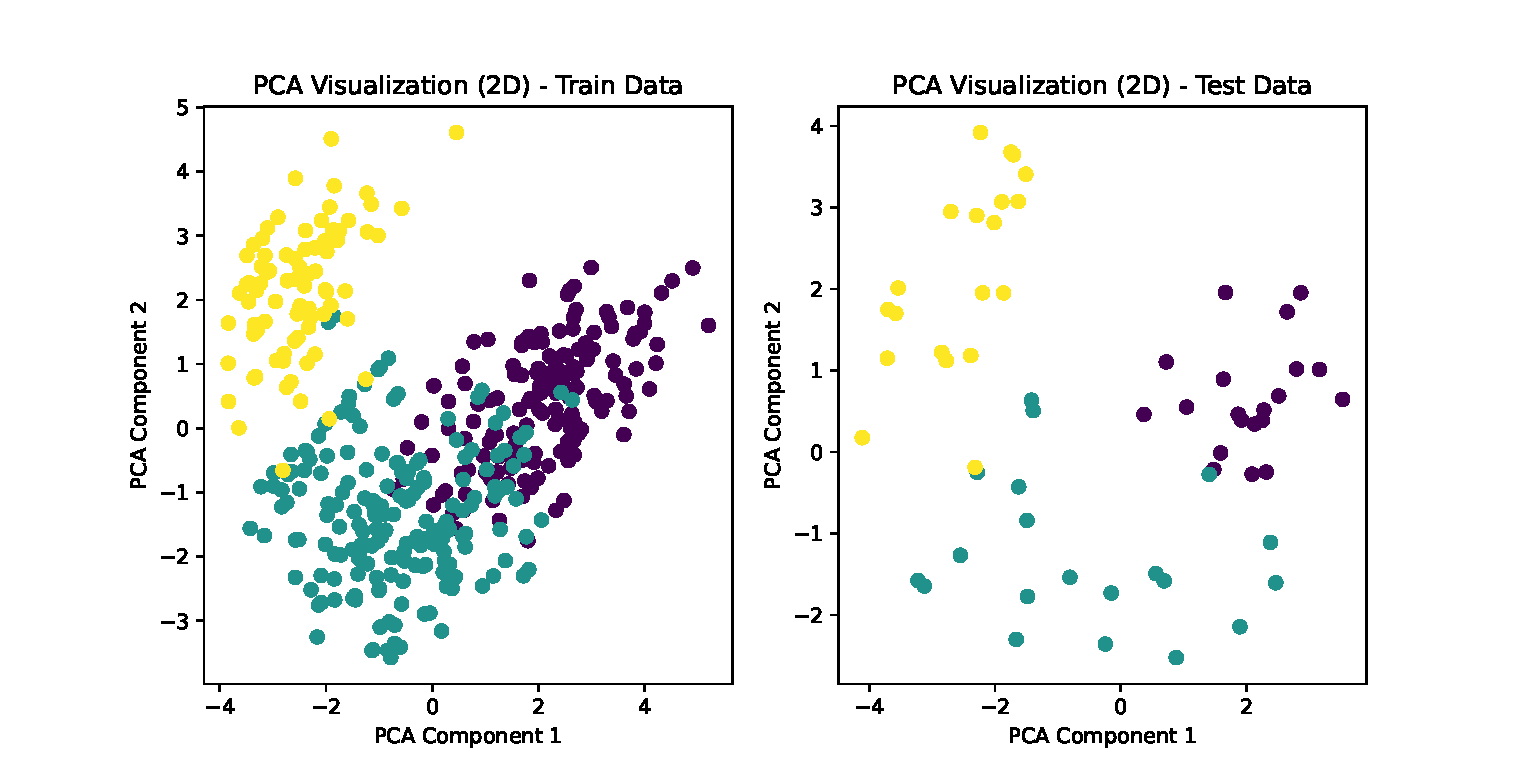
\includegraphics[scale=0.7]{2D_visualize.eps}
        \caption{2D visualization of the dataset.}
        \label{fig:2d_visual}
    \end{figure}
    \begin{figure}[H]
        \centering
        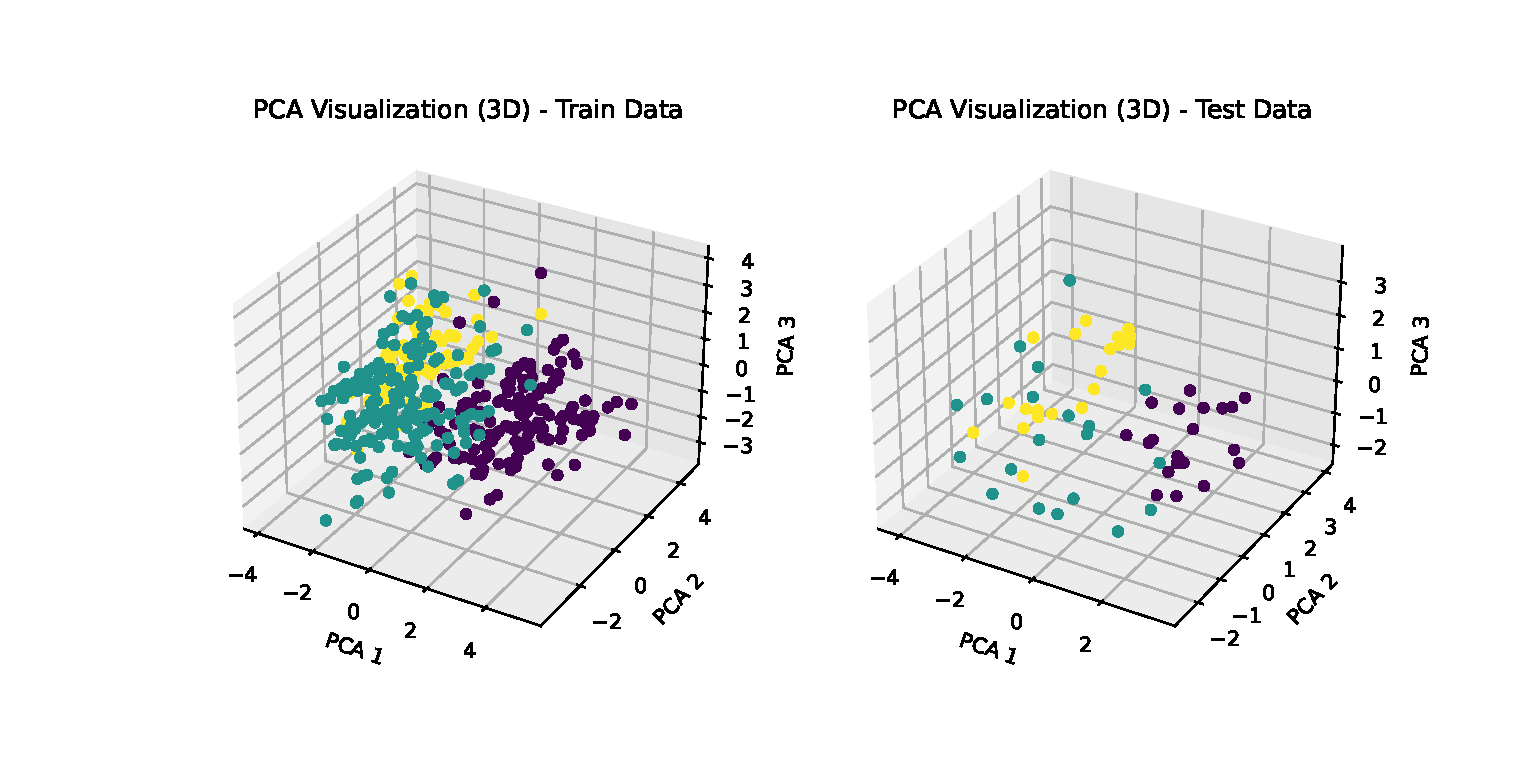
\includegraphics[scale=0.7]{3D_visualize.eps}
        \caption{3D visualization of the dataset.}
        \label{fig:3d_visual}
    \end{figure}
    
    \item \textbf{Effect of Prior Distribution:}  
    To evaluate the influence of prior probabilities on classification performance, 
    we \textcolor{blue}{implement a Maximum Likelihood (ML) classifier, which completely 
    disregards prior information}. The performance of the ML classifier is shown below:

    \begin{figure}[H]
        \centering
        \includegraphics[scale=1.0]{cm_ML.eps}
        \caption{Confusion matrix of the ML classifier.}
        \label{fig:cm_ml}
    \end{figure}

    Interestingly, \textcolor{blue}{the results are identical to those obtained with the
     MAP classifier}. 
    This is because, in this problem, the \textcolor{blue}{likelihood values are much 
    smaller than the prior probabilities}. Since the posterior probability is the product 
    of the likelihood and prior, the likelihood becomes the dominant factor, making the 
    effect of the prior negligible.

    \item \textbf{Contribution of Each Feature:}  
    To analyze the importance of each feature, we \textcolor{blue}{train the MAP classifier using all 
    features except one and measure the resulting accuracy}. A larger drop in accuracy indicates that
    the removed feature is more important for classification. The results are summarized in 
    Table~\ref{tab:feature_contribution}. The accuracy of the original MAP classifier is $95\%$.  
    It can be seen that when \textcolor{blue}{removing the first six features in Table~\ref{tab:feature_contribution}, 
    the accuracy decreases}, indicating that these features contribute positively to the classification 
    performance. On the other hand, \textcolor{blue}{removing the last few features leads to an increase
    in accuracy}, suggesting that these features introduce noise or redundant information rather than 
    aiding the classification.
    \begin{table}[h]
        \centering
        \begin{tabular}{|c|c|}
            \hline 
            \textbf{Feature Removed} & \textbf{Accuracy after remove the feature} \\ 
            \hline
            alcohol                         & $93.3\%$ \\  
            \hline 
            malic\_acid                     & $93.3\%$ \\  
            \hline 
            ash                             & $93.3\%$ \\
            \hline
            flavanoids                      & $93.3\%$ \\
            \hline
            hue                             & $93.3\%$ \\
            \hline
            od280/od315\_of\_diluted\_wines  & $93.3\%$ \\ 
            \hline 
            alcalinity\_of\_ash             & $95.0\%$ \\ 
            \hline
            magnesium                       & $95.0\%$ \\  
            \hline
            total\_phenols                   & $95.0\%$ \\  
            \hline
            nonflavanoid\_phenols            & $95.0\%$ \\  
            \hline
            proanthocyanins                 & $95.0\%$ \\  
            \hline
            proline                         & $95.0\%$ \\  
            \hline
            color\_intensity                 & $96.7\%$ \\  
            \hline
        \end{tabular}
        \caption{Table 1. Classification accuracy when removing each feature.}
        \label{tab:feature_contribution}
    \end{table}


    
\end{itemize}
